\documentclass[Royal,times,sageh]{sagej}

\usepackage{moreverb,url,natbib, multirow, tabularx}
\usepackage[colorlinks,bookmarksopen,bookmarksnumbered,citecolor=red,urlcolor=red]{hyperref}





\begin{document}

\title{Missing the Point: Non-Convergence in Iterative Imputation Algorithms}

\runninghead{Oberman}

\author{H. I. Oberman\affilnum{1}}

\affiliation{\affilnum{1}{Department of Methodology and Statistics, Utrecht University, Utrecht, The Netherlands}}

\corrauth{Hanne Oberman, Sjoerd Groenman building, Utrecht Science Park, Utrecht, The Netherlands.}

\email{\href{mailto:h.i.oberman@uu.nl}{\nolinkurl{h.i.oberman@uu.nl}}}

\begin{abstract}
Iterative imputation is a popular tool to accommodate missing data. While it is widely accepted that valid inferences can be obtained with this technique, these inferences all rely on algorithmic convergence. There is no consensus on how to evaluate the convergence properties of the method. This paper provides insight into identifying non-convergence of iterative imputation algorithms.
\end{abstract}

\keywords{missing data, iterative imputation, non-convergence, mice}

\maketitle

\hypertarget{introduction}{%
\section{Introduction}\label{introduction}}

Anyone who analyzes person-data may run into a missing data problem. Missing data is not only ubiquitous, but treating it can also be tedious. If a dataset contains just one incomplete observation, statistical inferences are undefined and will not produce any results. To circumvent this, many statistical packages employ list-wise deletion by default (i.e., ignoring incomplete observations). Unfortunately, this \emph{ad hoc} solution may yield wildly invalid results \citep{buur18}. An alternative is to \emph{impute} (i.e., fill in) the missing values in the incomplete observations. Subsequently, statistical inferences can be performed on the completed dataset. By repeating this process several times, a distribution of plausible results may be obtained, which reflects the uncertainty in the data due to missingness. This technique is known as `multiple imputation' \citep[MI;][]{rubin76}. MI has proven to be a powerful technique to draw valid inferences from incomplete data under many circumstances \citep{buur18}.

Figure \ref{fig:diagram} provides an overview of the steps involved with MI. Missing data \(y_{mis}\) in an incomplete dataset is imputed \(M\) times. The imputed data \(y_{imp}\) is combined with the observed data \(y_{obs}\) to create \(M\) completed datasets. On each completed dataset, an analysis of scientific interest is performed. The quantity of scientific interest (e.g., a regression coefficient) is denoted with \(Q\). Since \(Q\) is estimated on each completed dataset, \(M\) separate \(\hat{Q}\)-values are obtained. These \(M\) values are combined into a single pooled estimate \(\bar{Q}\). The premise of multiple imputation is that \(\bar{Q}\) is an unbiased and confidence valid estimate of the true---but missing---data inference.

\begin{figure}

{\centering 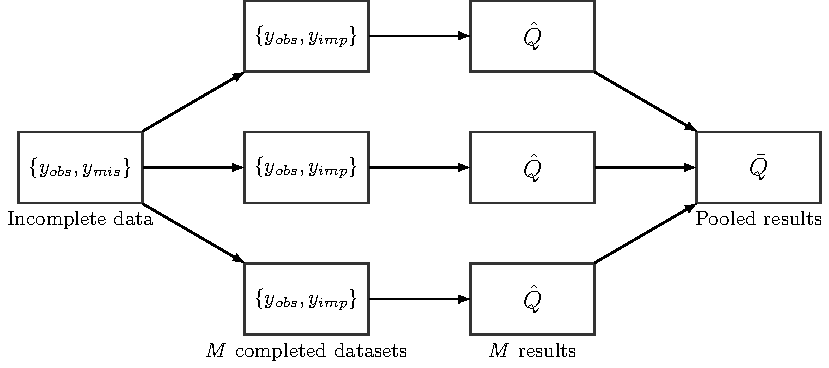
\includegraphics[width=\linewidth]{../Figures/diagram} 

}

\caption{Scheme of the main steps in multiple imputation (where $M=3$)---from an incomplete dataset, to $M$ multiply imputed datasets, to $M$ estimated quantities of scientific interest $\hat{Q}$s, to a single pooled estimate $\bar{Q}$.}\label{fig:diagram}
\end{figure}

A popular method to obtain imputations is to use the `Multiple Imputation by Chained Equations' algorithm, shorthand `MICE'\citep{mice}. With MICE, imputed values \(y_{imp}\) are drawn from the posterior predictive distribution of the missing values \(y_{mis}\). The algorithm is named after the iterative algorithmic procedure by which imputed values are generated: a multivariate distribution is obtained by iterating over a sequence of univariate imputations. The iterative nature of algorithms like MICE introduces a potential threat to the validity of the imputations: What if the algorithm has not converged? Are the implications then to be trusted? And can we rely on the inference obtained on the completed data? These are all open questions, because the convergence properties of iterative imputation algorithms have not been systematically studied \citep{buur18}. Moreover, there is no scientific consensus on how to evaluate convergence of imputation algorithms \citep{taka17}. Some default MICE techniques (e.g., `predictive mean modeling') might not yield converged states at all \citep{murr18}. Therefore, algorithmic convergence should be monitored carefully.

Currently, the recommended practice for evaluating the convergence of iterative imputation algorithms is through visual inspection. That is, the state space of the algorithm is monitored by plotting a scalar summary \(\theta\) against the iteration number.
\textbf{{[}Segway to WHAT TO MONITOR? Also, this paragraph is more or less the same as the third paragraph in the second section. Merge or remove one of the two?{]}} Typically, the \(\theta\)s under evaluation are chain means and variances (\textbf{define!}). These \(\theta\)s may be insufficient because they are summaries of the univariate state space of the algorithm, while MICE is not only concerned with univariate estimates, but the entire multivariate distribution of \(y_{imp}\). A suggestion by \citet{buur18} for a multivariate \(\theta\) to monitor is the quantity of scientific interest \(Q\) (e.g., a regression coefficient). Implementing this, however, might be somewhat advanced for empirical researchers. Moreover, this scalar summary is not model-independent, i.e., it only applies to one model of scientific interest. Yet, one of the advantages of MI is that the missing data problem and scientific problem are solved independently. Therefore, this \(\theta\) is not sufficient either. Van Buuren \citeyearpar[\(\S\) 4.5.2]{buur18} also proposed multivariable evaluation of the MICE algorithm through eigenvalue decomposition, building on the work of \citet{mack03}. Eigenvalues of a variance-covariance matrix are a measure of the data's total covariance. This would be a model-independent, multivariate scalar summary to monitor, but it has not yet been implemented.
\textbf{{[}Segway to HOW TO MONITOR?{]}} Monitoring convergence visually is insufficient on two counts: 1) it may be challenging to the untrained eye, and 2) only severely pathological cases of non-convergence may be diagnosed \citep[\(\S\) 6.5.2]{buur18}. Therefore, a quantitative, diagnostic evaluation of convergence would be preferred---although not straightforward. Iterative imputation algorithms such as MICE are Markov chain Monte Carlo (MCMC) methods. In MCMC methods, convergence is not from a scalar to a point, but from one distribution to another. The values generated by the algorithm (e.g., imputed values) will vary even after convergence \citep{gelm13}. Since MCMC algorithms do not reach a unique point at which convergence is established, diagnostics may only identify signs of \emph{non}-convergence \citep{hoff09}. Several of such non-convergence diagnostics exist, but it is not known whether these are appropriate for iterative imputation algorithms.

In this paper, we investigate how non-convergence in iterative imputation algorithms may be diagnosed. First, we define which non-convergence diagnostics will be considered, and evaluate how these diagnostics could be appropriate for iterative imputation applications. In the second part of this paper, we will investigate the impact of inducing non-convergence in iterative imputation algorithms by means of model-based simulation in \texttt{R} \citep{R}. The aim of the simulation is to determine whether unbiased, confidence valid inferences may be obtained under different levels of non-convergence (\textbf{and at which point convergence may safely be assumed}). Additionally, we will assess how well different non-convergence diagnostics perform in identifying signs of non-convergence (\textbf{and on which scalar summary of the state space of the algorithm these diagnostics should be applied}). The results of this study are guidelines for identifying non-convergence in iterative imputation algorithms, which will aid applied researchers in drawing valid inference from incomplete datasets. \textbf{{[}add more societal relevance: what is the consequence of non-convergence? see example of non-convergence in Figure 2 (e.g., biased estimates, invalid inference, etc.){]}} For reasons of brevity, we only focus on the iterative imputation algorithm implemented in the popular \texttt{mice} package \citep{mice} in \texttt{R} \citep{R}.

\textbf{{[}Include sub-questions and make structure of the paper clear!{]}} How can non-convergence be identified diagnostically? Are common MCMC non-convergence diagnostics appropriate for MICE? And if so, which threshold should be used to diagnose non-convergence? How many iterations are sufficient/needed to be able to diagnose non-convergence? Are the default number of iterations sufficient (i.e., 5 in mice, 10 in SPSS and Stata, 30 in mi)? How severe is it when the algorithm has not converged? And what are guidelines for practice? Can the parameter of interest \(Q\) be correct when the algorithm is not (yet) converged, and vice versa?

\hypertarget{some-notation}{%
\subsection{Some notation}\label{some-notation}}

Let \(y\) denote an \(n \times k\) matrix containing the data values on \(k\) variables for all \(n\) units in a sample. The data value of unit \(i\) (\(i = 1, 2, \dots, n\)) on variable \(j\) (\(j = 1, 2, \dots, k\)) may be either observed or missing. The number of units \(i\) in dataset \(y\) with at least one missing value, divided by the total number of units \(n\), is called the missingness proportion \(p_{mis}\). The collection of observed data values in \(y\) is denoted by \(y_{obs}\); the missing part of \(y\) is referred to as \(y_{mis}\). For each datapoint in \(y_{mis}\), we sample \(M \times T\) plausible values, where \(M\) is the number of imputations (\(m = 1, 2, \dots, M\)) and \(T\) is the number of iterations (\(t = 1, 2, \dots, T\)) in the imputation algorithm. The collection of samples between the initial value (at \(t=1\)) and the final imputed value (at \(t=T\)) will be referred to as an `imputation chain'. \textbf{{[}If not defined elsewhere, add: \(\theta\)s are scalar summaries of the algorithm at a certain iteration (e.g., chain means; the average of the imputed values in each imputation chain).{]} }

\hypertarget{identifying-non-convergence}{%
\section{Identifying non-convergence}\label{identifying-non-convergence}}

There are two requirements for convergence of iterative algorithms: mixing and stationarity \citep{gelm13}. Without mixing, imputation chains do not intermingle nicely, indicating that the distribution of imputed values differs across imputations. Chains may be `stuck' at a local optimum, instead of sampling imputed values from the entire predictive posterior distribution of the missing values. This may cause under-estimation of the variance within chains, which results in spurious, invalid inferences. Without stationarity, there is trending within imputation chains. Trending implies that further iterations would yield a different set of imputations. Iterative imputation algorithms that have not yet reached stationarity, may thus yield biased estimates.

\textbf{{[}Move to INTRO???{]}} To illustrate what non-convergence looks like in iterative imputation algorithms, we reproduce an example from van Buuren \citeyearpar[\(\S\) 6.5.2]{buur18}. Figure \ref{fig:non-conv} displays a subset of the example: a variable that we will call \(j\). We see two traceplots of the chain means for \(j\)---i.e., the average of the imputed values for \(j\) in each imputation \(y_{imp,m}\), plotted against the iteration number. Each line portrays one imputation. The plot on the left-hand side of the figure shows typical convergence of an iterative imputation algorithm. The right-hand side displays pathological non-convergence, induced by purposefully mis-specifying the imputation model. \textbf{{[}Leave this in if it's after mixing and stationarity are defined, otherwise remove?{]} In the typical convergence situation, the imputation chains intermingle nicely and there is little to no trending. In the non-convergence plot, there is a lot of trending and some chains do not intermingle.} Importantly, the chain means at the last iteration (the imputed value per \(m\)) are very different between the two plots. The algorithm with the mis-specified model yields imputed values that are on average a factor two larger than those of the typically converged algorithm. That means that non-convergence has a impact on the mean of \(j\) in \(y_{imp, m}\). This difference (presumably) translates to bias in the \(M\) completed data estimates \(\hat{\mu}_{j,m}\), and consequently also to the pooled estimate \(\bar{\mu}_j\). Non-convergence thus leads to biased estimates. This shows the importance of reaching converged states in iterative imputation algorithms.

\begin{figure}

{\centering 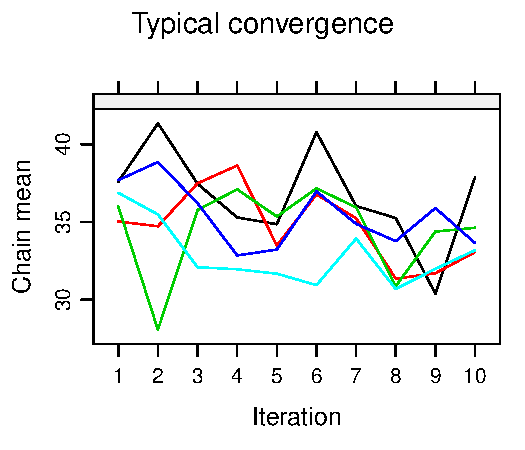
\includegraphics[width=.49\linewidth]{2.Manuscript_files/figure-latex/non-conv-1} 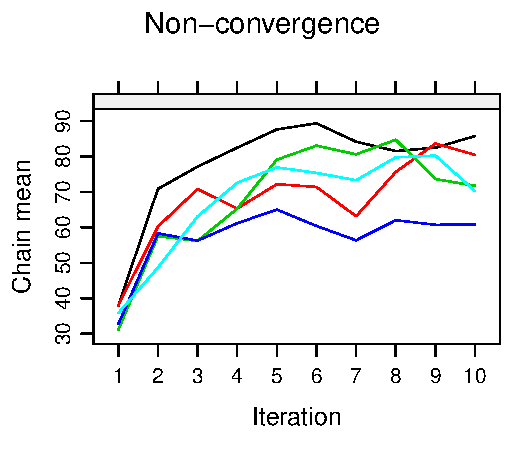
\includegraphics[width=.49\linewidth]{2.Manuscript_files/figure-latex/non-conv-2} 

}

\caption{Typical convergence versus pathological non-convergence. Please note that this is the same data with a different imputation model, leading to different imputations (e.g., see the units on the y-axis).}\label{fig:non-conv}
\end{figure}

\textbf{{[}Move to INTRO???{]}} Convergence has historically been inspected visually, by monitoring the imputation algorithm over iterations. This is typically done through traceplots. In a traceplot, the iteration number is plotted against a certain \(\theta\). \(\theta\)s are scalar summaries of the state space of the algorithm at a specific iteration. The recommended scalar summaries to evaluate are chain means and chain variances. Additionally, researchers may ``monitor some statistic of scientific interest'' \citep[\(\S\) 6.5.2]{buur18}. As \citet{buur18} describes, researchers can specify their quantity of scientific interest \(Q\) (e.g., a regression coefficient) as scalar summary \(\theta\). Such a user-defined scalar summary, however, may be somewhat advanced for empirical researchers. And moreover, it is not universal to all complete data problems. Focusing on the convergence of outcome parameters may influence the iterative imputation procedure in the sense that the model of evaluation favors the model of interest. The downside to these two approaches is that they either focus on the univariate state space, or primarily track the change over the iterations of a multivariate outcome conform the scientific model of interest. Ideally, one would like to evaluate a model-independent parameter that summarizes the multivariate nature of the data. Therefore, we propose a \(\theta\) that summarizes the multivariate state space of the algorithm, but is independent from the model of scientific interest. We propose \(\lambda_1\) as such a scalar summary. We define \(\lambda_1\) as the first eigenvalue of the variance-covariance matrix of the completed data. Let \(\lambda_1 \geq \lambda_2 \geq ... \geq \lambda_j\) be the eigenvalues of \(\Sigma\) in each of the \(M\) completed datasets \({y_{obs}, y_{imp}}\). \(\lambda_1\) is measure that summarizes the covariances in the completed datasets. \textbf{The first eigenvalue has the appealing property that is not dependent on the substantive model of interest. Eigenvalue decomposition is inspired by \citet{mack03}.}

\hypertarget{diagnostics-under-evaluation}{%
\subsection{Diagnostics under evaluation}\label{diagnostics-under-evaluation}}

Non-convergence diagnostics for MCMC algorithms typically identify problems in either one of the two requirements for convergence: mixing or stationarity. Non-stationarity within chains may be diagnosed with e.g., autocorrelation \citep[\(AC\);][]{scha97, gelm13}, numeric standard error \citep[`MC error';][]{gewe92}, or Raftery and Lewis's \citeyearpar{raft91} procedure to determine the effect of trending on the precision of estimates. A widely used diagnostic to monitor mixing between chains is the potential scale reduction factor \(\widehat{R}\) \citep[`Gelman-Rubin statistic';][]{gelm92}. With a recently proposed adaptation, \(\widehat{R}\) might also serve to diagnose non-stationarity, but this has not yet been thoroughly investigated \citep{veht19}. Therefore, we use \(\widehat{R}\) and \(AC\) to evaluate mixing and stationarity separately, as recommended by e.g., \citet{cowl96}.

\textbf{{[}Add: effective sample size is used if we want independent samples \emph{within} chains. In MI, we only use the final estimate. Also, computing n\_eff assumes infinitely many iterations, which is fine in Bayesian analyses where T is often at least one thousand. But the default in iterative imp is often substantially lower.{]}}

\hypertarget{potential-scale-reduction-factor}{%
\subsubsection{Potential scale reduction factor}\label{potential-scale-reduction-factor}}

The potential scale reduction factor \(\widehat{R}\) was coined by \citet{gelm92}. An updated version of \(\widehat{R}\) has been proposed by Vehtari et al.~\citeyearpar[p.~5]{veht19}. \textbf{This version is better suited to detect non-convergence in the tails of distributions, by using three transformations on the scalar summary that it is applied to. Namely, rank-normalization, folding, and localization. The Vehtari et al.~version of \(\widehat{R}\) may be suitable for iterative imputation. We therefore use their definition of the diagnostic.} Let \(M\) be the total number of chains, \(T\) the number of iterations per chain, and \(\theta\) the scalar summary of interest (e.g., chain means). For each chain (\(m = 1, 2, \dots, M\)), we estimate the variance of \(\theta\), and average these to obtain within-chain variance \(W\).

\begin{align*}
W&=\frac{1}{M} \sum_{m=1}^{M} s_{j}^{2}, \text { where } s_{m}^{2}=\frac{1}{T-1} \sum_{t=1}^{T}\left(\theta^{(t m)}-\bar{\theta}^{(\cdot m)}\right)^{2}. 
\end{align*}

\noindent We then estimate between-chain variance \(B\) as the variance of the collection of average \(\theta\) per chain.

\begin{align*}
B&=\frac{T}{M-1} \sum_{m=1}^{M}\left(\bar{\theta}^{(\cdot m)}-\bar{\theta}^{(\cdot \cdot)}\right)^{2}, \text { where } \bar{\theta}^{(\cdot m)}=\frac{1}{T} \sum_{t=1}^{T} \theta^{(t m)} \text{, } \bar{\theta}^{(\cdot \cdot)}=\frac{1}{M} \sum_{m=1}^{M} \bar{\theta}^{(\cdot m)}. 
\end{align*}

\noindent From the between- and within-chain variances we compute a weighted average, \(\widehat{\operatorname{var}}^{+}\), which approximates the total variance of \(\theta\). \(\widehat{R}\) is then obtained as a ratio between the total variance and the within-chain variance:

\begin{equation*}
\widehat{R}=\sqrt{\frac{\widehat{\operatorname{var}}^{+}(\theta | y)}{W}},
\text{ where } \widehat{\operatorname{var}}^{+}(\theta | y)=\frac{N-1}{N} W+\frac{1}{N} B.
\end{equation*}

We can interpret \(\widehat{R}\) as potential scale reduction factor since it indicates by how much the variance of \(\theta\) could be shrunken down if an infinite number of iterations per chain would be run \citep{gelm92}. This interpretation assumes that chains are `over-dispersed' at \(t=1\), and reach convergence as \(T \to \infty\). Over-dispersion implies that the initial values of the chains are `far away' from the target distribution and each other. When the sampled values in each chain are independent of the chain's initial value, the mixing component of convergence is satisfied. The variance between chains is then equivalent to the variance within chains, and \(\widehat{R}\)-values will be close to one. High \(\widehat{R}\)-values thus indicate non-convergence. The conventionally acceptable threshold for convergence was \(\widehat{R} < 1.2\) \citep{gelm92}. More recently, \citet{veht19} proposed a more stringent threshold of \(\widehat{R} < 1.01\).

\hypertarget{autocorrelation}{%
\subsubsection{Autocorrelation}\label{autocorrelation}}

Following the same notation, we define autocorrelation as the correlation between two subsequent \(\theta\)-values within the same chain \citep[p.~147]{lync07}. In this study, we only consider \(AC\) at lag 1, i.e., the correlation between the \(t^{th}\) and \(t+1^{th}\) iteration of the same chain.

\begin{equation*}
AC = \left( \frac{T}{T-1} \right) \frac{\sum_{t=1}^{T-1}(\theta_t - \bar{\theta}^{(\cdot m)})(\theta_{t+1} - \bar{\theta}^{(\cdot m)})}{\sum_{t=1}^{T}(\theta_t - \bar{\theta}^{(\cdot m)})^2}.
\end{equation*}

We can interpret \(AC\)-values as a measure of stationarity. If \(AC\)-values are close to zero, there is no dependence between subsequent samples within imputation chains. Negative \(AC\)-values indicate divergence within imputation chains. \textbf{Subsequent sampled values within each imputation chain are less alike.} Positive \(AC\)-values indicate recurrence. If \(\theta\)-values of subsequent iterations are similar, trending may occur. Negative \(AC\)-values show no threat to the stationarity component of convergence. On the contrary even---negative \(AC\)-values indicate that \(\theta\)-values of subsequent iterations diverge from one another, which may increase the variance of \(\theta\) and speed up convergence. As convergence diagnostic, the interest is therefore in positive \(AC\)-values. The magnitude of \(AC\)-values may be evaluated statistically, using a Wald test with \(AC=0\) as null hypothesis \citep{box15}.

\hypertarget{thresholds}{%
\subsubsection{Thresholds}\label{thresholds}}

Upon convergence, \(\widehat{R}=1\) and \(AC=0\), which are unlikely thresholds for MCMC algorithms, because of its convergence to a distribution. Even in the most converged state, the algorithm will show some signs of non-mixing and non-stationarity. Upon \emph{sufficient} convergence, the imputation chains will intermingle such that the only difference between the chains is caused by the randomness induced by the algorithm (\(\widehat{R} > 1\)), and there may be some dependency between subsequent iterations of imputation chains (\(AC > 0\)). In practice, non-convergence is usually diagnosed when \(\widehat{R}\) \textgreater{} 1.2 or 1.1 or even 1.01. And a t-test is performed to assess whether \(AC\) is significantly different from zero.

\hypertarget{in-practice}{%
\subsection{In practice}\label{in-practice}}

Before we evaluate the performance of the non-convergence diagnostics \(\widehat{R}\) and \(AC\) quantitatively through simulation, we apply them to the example of pathological non-convergence by \citet{buur18} that we reproduced above. We want to be able to draw the same conclusions as we did from visually inspecting the two algorithms. But \(\widehat{R}\) and \(AC\) should at least be able to distinguish between the two algorithms plotted in Figure \ref{fig:non-conv}. From visual inspection, we know that the typically converged algorithm initially portrayed some signs of non-mixing (around \(t=2\)), but intermingled nicely overall. Additionally, there was very little trending. The algorithm with pathological non-convergence showed severe non-mixing, although this gradually improved (from \(t=7\)). Moreover, there was a lot of trending as well initially (up-to \(t=6\)), after which the chains reached a somewhat more stationary state. To assess whether \(\widehat{R}\) and \(AC\) may be appropriate non-convergence identifiers for iterative imputation algorithms, they should identify the same trends as the visual inspection. But at least, the following condition must hold: the methods should indicate worse performance for the mis-specified model with pathological non-convergence than the typically converged algorithm (i.e., higher \(\widehat{R}\)- and \(AC\)-values).

In Figure \ref{fig:diagnostics}A, the chain means from Figure \ref{fig:non-conv} are plotted again---now together. Panel B shows two versions of calculating \(AC\)s applied to the \(\theta\)s of panel A: the default calculation with \texttt{R} function \texttt{stats::acf()} \citep{R}, and manual calculation as the correlation between \(\theta\) in iteration \(t\) and \(\theta\) in iteration \(t+1\). Panel C shows the traditional computation of \(\widehat{R}\), and panel D shows \(\widehat{R}\) as computed by implementing \citet{veht19} 's recommendations. \textbf{{[}Add labels for the two types of Rhat to the figure!{]}}

\begin{figure}

{\centering 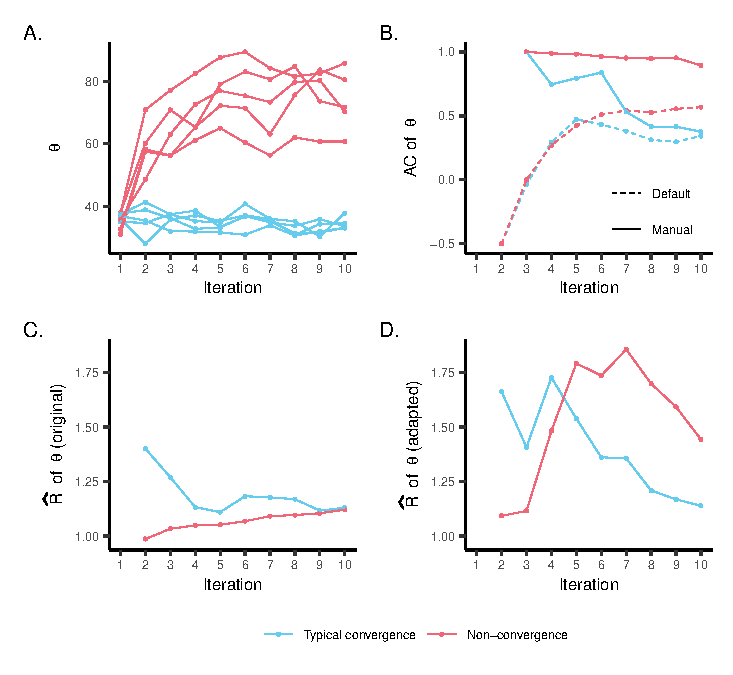
\includegraphics{2.Manuscript_files/figure-latex/diagnostics-1} 

}

\caption{Convergence diagnostics applied on the imputation algorithms of Figure 2. $\theta$ = chain mean in $y_{imp, m}$.}\label{fig:diagnostics}
\end{figure}

When we look at panel B, we conclude something weird. The \(AC\)-values calculated with the default function indicate equal performance for the typical convergence and the pathological non-convergence (up-to \(t=5\)), while there is obvious trending in the \(\theta\)s of the latter. Moreover, the best convergence (as indicated by the lowest \(AC\)-value) is observed at \(t=2\), but looking at the chain means in panel A, there should be some signs of trending up-to iteration number seven. After consulting the documentation on \texttt{stats::acf()} \citep{R}, we conclude that this \(AC\) function is not suited for iterative imputation algorithms. The function is optimized for performance when \(t\geq50\) \citep{box15}, while the default number of iterations in iterative imputation is often much lower. Therefore, we compute \(AC\) manually, see the solid line. These \(AC\) values indicate non-stationarity as expected. We therefore calculate \(AC\) manually.

\textbf{Describe panel C here and why it is not optimal{]}} The \(\widehat{R}\)-values in panel D do meet the requirements specified above. \(\widehat{R}\) as computed conform \citet{veht19} does indeed indicate less signs of non-convergence as the number of iterations goes up. \textbf{\citep[explain the dip in Rhat values at t=2. Namely, because we can only use 2 of the 3 tricks by][ if the number of iterations is very low (t\textless4). That's why the \(\widehat{R}\)s are more similar to the traditional GR.]{veht19}}

\textbf{In conclusion, we will use \(\widehat{R}\) conform \citet{veht19} and \(AC\) computed manually as non-convergence diagnostics in the simulation study. The diagnostics will be applied to four \(\theta\)s of interest: chain means, chain variances, a quantity of scientific interest, and the first eigenvalue of the variance-covariance matrix.}

\hypertarget{simulation-study}{%
\section{Simulation study}\label{simulation-study}}

The aim of the simulation study is to evaluate the impact of inducing non-convergence in the MICE algorithm on several quantities of scientific interest \(Q\). Subsequently we will evaluate how well \(\widehat{R}\) and \(AC\) perform in identifying the effects of non-convergence \textbf{{[}and performance of different thetas{]}}. And finally, we will formulate an informed advice on the requirements to safely assume \emph{sufficient} convergence in practice. That is, we assume that the algorithm is \emph{sufficiently} converged when each estimate \(\bar{Q}\) is an unbiased and confidence valid estimate of the corresponding estimand \(Q\). \textbf{{[}and formulate advice on thetas?{]}}

Non-convergence will be induced by: 1) increasing the missingness proportion \(p_{mis}\) in dataset \(y\) incrementally, and 2) terminating the imputation algorithm at a varying number of iterations \(T\). The first set of simulation conditions---the missingness proportions---is chosen to reflect the difficulty of the missingness problem. The underlying assumption is that low missingness proportions lead to quick algorithmic convergence, since there is a lot of information in the observed data. Higher missingness proportions should yield slower convergence. Unless, however, the fraction of missing information is so high that the random component in the imputation algorithm outweighs the information in the observed data. Then, convergence to a stable but highly variable state may be reached instantaneously. We assume that the incremental missingness proportions in our study will result in a corresponding increase in signs of non-convergence.

The assumption inherent to the second set of simulation conditions---the number of iterations---is that terminating the imputation algorithm too early causes non-convergence. Generally, the algorithm will not reach convergence if \(T=1\), because the imputed values in the first iteration (at \(t=1\)) depend on the initial values of the algorithm (which are sampled randomly from the set of observed datapoints). As the number of iterations increases, the imputation chains should become independent of the initial values, until the point at which adding an extra iteration does not lead to a more converged state. We assume that we can induce non-convergence at least in conditions where \(T\) is smaller than the default number of iterations in \texttt{mice}, \(T=5\).

\hypertarget{hypotheses}{%
\subsection{Hypotheses}\label{hypotheses}}

\begin{enumerate}
\def\labelenumi{\arabic{enumi}.}
\item
  We expect that simulation conditions with a high missingness proportion \(p_{mis}\) and a low number of iterations \(T\) will result in biased, invalid estimates of the quantities of scientific interest, \(Q\)s.
\item
  We hypothesize that \(\widehat{R}\) and \(AC\) will correctly identify signs of non-convergence in those simulation conditions where the \(\bar{Q}\)s are \emph{not} unbiased and confidence valid estimates of the \(Q\)s.
\item
  We hypothesize that the recommended thresholds to diagnose non-convergence with \(\widehat{R}\) (\(\widehat{R} > 1.2\), \(\widehat{R} > 1.1\), and \(\widehat{R} > 1.01\)) may be too stringent for iterative imputation applications. In an empirical study, where \(\widehat{R}\) was used to inform the required imputation chain length, it took as many as 50 iterations to overcome the conventional non-convergence threshold \(\widehat{R}>1.2\). Yet, scientific estimates were insensitive to continued iteration from \(t=5\) onward \citep{lace07}. We therefore suspect that \(\widehat{R}\) may over-estimate signs of non-convergence in iterative imputation algorithms, compared to the validity of estimates. In contrast to this, it may occur that signs of non-convergence are under-estimated by \(\widehat{R}\), in exceptional cases where the initial values of the algorithm are not appropriately over-dispersed \citep[p.~437]{broo98}. In e.g.~\texttt{mice}, initial values are chosen randomly from the observed data, hence we cannot be certain of over-dispersion in the initial values. In practice, we do not expect this to cause problems for identifying non-convergence with \(\widehat{R}\).
\item
  We expect that high \(AC\) values are implausible in iterative imputation algorithms with typical convergence. That is, after only a few iterations, the randomness induced by the algorithm should effectively mitigate the risk of dependency within chains.
\item
  \textbf{{[}Something about thetas, that multivariate thetas are better at detecting non-convergence than univariate thetas. The non-convergence diagnostics applied on the chain means and chain variances will fail to identify signs of non-convergence when the multivariate Qs are affected.{]}}
\end{enumerate}

\hypertarget{set-up}{%
\subsection{Set-up}\label{set-up}}

We investigate non-convergence of the MICE algorithm through model-based simulation in \texttt{R} \citep[version 3.6.3;][]{R}. The number of simulation repetitions is 1000. The simulation set-up is summarized in the pseudo-code below. The complete \texttt{R} script of the simulation study is available from \href{https://github.com/gerkovink/shinyMice/tree/master/3.Thesis/1.SimulationStudy}{github.com/gerkovink/shinyMice}.

\begin{verbatim}
# pseudo-code of simulation 
1. simulate data 
for (number of simulation runs from 1 to 1000)
 for (missingness proportions 5%, 25%, 50%, 75% and 95%)
  2. create missingness
  for (number of iterations from 1 to 100)
   3. impute missingness
   4. perform analysis of scientific interest
   5. compute non-convergence diagnostics 
   6. pool results across imputations
   7. compute performance measures
 8. combine outcomes of all missingness proportions
9. aggregate outcomes of all simulation runs 
\end{verbatim}

\hypertarget{data-generating-mechanism.}{%
\subsubsection{Data-generating mechanism.}\label{data-generating-mechanism.}}

In this study, sampling variance is not of interest. Therefore, a single complete dataset may serve as comparative truth in all simulation repetitions \citep{vink14}. The data-generating mechanism is a multivariate normal distribution, representing person-data on three predictor variables in a multiple linear regression problem \textbf{(from an unspecified social scientific field of study)}. Let the predictor space be defined as
\[
\begin{aligned}
\begin{pmatrix}X_1\\
X_2\\
X_3
\end{pmatrix} \sim \mathcal{N}
\begin{bmatrix}
\begin{pmatrix}
12\\
3\\
0.5
\end{pmatrix}\!\!,
\begin{pmatrix}
4 & 4 & 1.8 & 0\\
4 & 16 & 4.8 & 0\\
1.8 & 4.8 & 9 & 0
\end{pmatrix}
\end{bmatrix}\!\!\text{.}\\[2\jot]
\end{aligned}
\]
A finite population of \(N=1000\) is simulated using the \texttt{mvtnorm} package \citep{mvtnorm}. Subsequently, a fourth variable is constructed as outcome \(Y\). For each unit \(i = 1, 2,..., N\), let
\[
Y_i = 1 + 2X_{1i} +.5X_{2i} - X_{3i} + \epsilon_i ,
\]
where \(\epsilon \sim \mathcal{N}(0, 100)\). From the complete set, we obtain the true values of several quantities of scientific interest, \(Q\)s. \textbf{{[}MOVE this next part to the start of the Simulation Study section?{]} \(Q\)s are the targets that will be estimated in each simulation repetition, after first \emph{amputing} the complete data with varying missingness proportions, then imputing the missingness with a varying number of iterations, then estimating the \(Q\)s on the \(M\) completed datasets, and finally pooling the \(M\) estimates \(\hat{Q}\) to obtain a single \(\bar{Q}\) for each \(Q\). We try to predict the effect of non-convergence (i.e., the difference between \(Q\) and \(\bar{Q}\)) with the convergence diagnostics \(\widehat{R}\) and \(AC\), by applying these methods to several scalar summaries of the state space of the algorithm, \(\theta\)s.}

\hypertarget{scientific-estimands.}{%
\subsubsection{Scientific estimands.}\label{scientific-estimands.}}

We consider four types of \(Q\)s that are often of interest in empirical research. Namely, two descriptive statistics: the mean \(\mu_j\) and standard deviation \(\sigma_j\) of each variable \(j = Y, X_1, X_2, X_3\). We also consider the regression coefficients of the predictors: \(\beta_1\), \(\beta_2\), and \(\beta_3\) in regression equation
\[Y' = \beta_0 + \beta_1 X_1 + \beta_2 X_2 + \beta_3 X_3,\]
where \(Y'\) is the expected value of the outcome. And finally, the proportion of variance explained by the set of predictors: coefficient of determination \(r^2 \times 100\) \textbf{(note that lower case \(r\) is used to avoid confusion with non-convergence diagnostic \(\widehat{R}\))}. The true values of these scientific estimands are calculated on the complete data with the \texttt{R} functions \texttt{base::mean()}, \texttt{stats::sd()}, and \texttt{stats::lm()} \citep{R}.

\hypertarget{methods.}{%
\subsubsection{Methods.}\label{methods.}}

In each simulation repetition, we \emph{ampute} the complete dataset five times to obtain five different incomplete datasets, \(y\)s. The ratio between \(y_{obs}\) and \(y_{mis}\) in each \(y\) depends on the missingness proportion: \(p_{mis} =.05,.25,.5,.75,.95\). We ampute the complete data with the \texttt{mice} package \citep[function \texttt{mice::ampute()};][]{mice}. We consider all possible univariate and multivariate patterns of missingness, conform a `missing completely at random' missingness mechanism \citep{rubin87}. I.e., the probability to be missing is the same for all \(N \times k\) cells in \(y\), conditional on the missingness proportion \(p_{mis}\).

Missing datapoints in each incomplete dataset \(y\) are imputed with the \texttt{mice()} function \citep{mice}. All imputation procedures are performed with Bayesian linear regression imputation, and five imputation chains (\(M=5\)). Because \(M=5\), each run of the \texttt{mice()} function results in five sets of imputations: \(y_{imp,m}\), where \(m = 1, 2, ..., 5\). The number of iterations in each run of the algorithm varies between simulation conditions (\(T=1,2,...,100\)).

From the 5 imputations \(y_{imp,m}\) we obtain the chain means and chain variances for each variable \(j\). These will serve as scalar summary \(\theta\) to apply non-convergence diagnostics \(\widehat{R}\) and \(AC\) on. We then use \texttt{mice::complete()} to combine the imputed data \(y_{imp,m}\) with the observed data \(y_{obs}\), resulting in five completed datasets \{\(y_{obs}, y_{imp, m}\)\}.

On the 5 completed datasets \{\(y_{obs}, y_{imp, m}\)\}, we:

\begin{itemize}
\item
  Estimate \(\hat{Q}\)s for \(Q= \mu\) and \(Q=\sigma\) with \texttt{base::mean()}, and \texttt{stats::sd()} \citep{R}. We pool the \(\hat{Q}\)s with \texttt{base::mean()} to get \(\bar{Q}\)s.
\item
  Compute \(\lambda_1\), to use as \(\theta\) in the two convergence diagnostics. By definition, the first eigenvalue of the variance-covariance matrix, \(\lambda_1\), is equal to the variance of the principal component solution of each \{\(y_{obs}, y_{imp, m}\)\}, which we calculate with \texttt{stats::princomp()} \citep{R}.
\item
  Perform multiple linear regression with \texttt{stats::lm()} \citep{R} to get the \(\hat{Q}\)s for \(Q=\beta\) and \(Q=r^2\). We pool the \(\hat{Q}\)s conform \citet{vink14} to get \(\bar{Q}\)s for the \(\beta\)s and \(r^2\) \textbf{{[}check finite pooling of \(r^2\), instead of \texttt{mice::pool.r.squared()}{]}}. Additionally, we use the \(\hat{Q}\)s of \(Q=\beta\) as \(\theta\) to apply the convergence diagnostics to.
\end{itemize}

We apply non-convergence diagnostics \(\widehat{R}\) and \(AC\) to each scalar summary \(\theta\). We calculate \(\widehat{R}\) by implementing Vehtari et al.'s \citeyearpar{veht19} recommendations, and \(AC\) as the correlation between the \(t^{th}\) and the \((t+1)^{th}\) iteration.

\hypertarget{performance-measures.}{%
\subsubsection{Performance measures.}\label{performance-measures.}}

We assess the impact of inducing non-convergence in the iterative imputation algorithm by comparing \(\bar{Q}\)s with \(Q\)s. For each \(Q\), we calculate bias as \(\bar{Q} - Q\). For the regression coefficients \(Q=\beta_{1,2,3}\), we also compute the empirical coverage rate (CR). CR is defined as the percentage of simulation repetitions in which the 95\% confidence interval (CI) around \(\bar{Q}\) covers the true estimand \(Q\). Let
\[\text{CI} = \bar{Q} \pm t_{(M-1)} \times SE_{\bar{Q}},\]
where \(t_{(M-1)}\) is the quantile of a \(t\)-distribution with \(M-1\) degrees of freedom, and \(SE_{\bar{Q}}\) is the square root of the pooled variance estimate. If we obtain nominal coverage (CR = 95\%), we can conclude that the \(\bar{Q}\)s are confidence valid estimates of the \(Q\)s. Finally, we inspect CI width (CIW): the difference between the lower and upper bound of the 95\% confidence interval around \(\bar{Q}\). CIW is of interest because too short CIs indicate under-estimation of the variance in \(\bar{Q}\), which may yield spurious inferences.

With these performance measures, we also evaluate how well the non-convergence diagnostics \(\widehat{R}\) and \(AC\) can identify simulation conditions in which the \(\bar{Q}\)s are \emph{not} unbiased, confidence valid estimates of the \(Q\)s. \textbf{{[}Rephrase this:{]} We measure the performance of \(\widehat{R}\) and \(AC\) by the four scalar summaries \(\theta\): chain means (i.e., the mean in each \(y_{imp, m, j}\)) versus \(Q=\mu\), chain variances (i.e., the variance in each \(y_{imp, m, j}\)) versus \(Q=\sigma\), the estimated regression coefficients \(\beta\) in each \{\(y_{obs}, y_{imp, m}\)\} (i.e., a user-defined statistic of scientific interest \(\hat{Q}\)) against \(Q=\beta\), and the first eigenvalue of the variance-covariance matrix in each \{\(y_{obs}, y_{imp, m}\)\}, \(\lambda_1\) versus \(Q=r^2\).}

\textbf{{[}Remove this?{]} Primarily, we want to know what the effect is of inducing non-convergence on the estimated \(Q\)s. More specifically, we are interested in the bias of \(\bar{Q}\) for all \(Q\)s and the confidence validity of \(\bar{Q}\) for \(Q=\beta\). Therefore, we evaluate these performance measures against the simulation conditions (the number of iterations \(T\) and the missingness proportion \(p_{mis}\)). We look at averages across simulation repetitions. Secondly, we want to know if conditions in which the \(Q\)s are affected by non-convergence are also identified by the non-convergence diagnostics \(\widehat{R}\) and \(AC\). We do this, again, by looking at the performance measures for the \(Q\)s, but now we evaluate these against what \(\widehat{R}\) and \(AC\) indicate about signs of non-convergence in the \(\theta\)s.}

\hypertarget{results}{%
\section{Results}\label{results}}

\textbf{{[}Add to this section: 1) emphasize that the iterations in the plots are averages across repetitions, not within one run of MICE; 2) Add more info about figure legends and axes{]}}

Our results show the impact of inducing non-convergence in an iterative imputation algorithm on several scientific estimates, and whether the non-convergence diagnostics \(\widehat{R}\) and \(AC\) identify the signs of non-convergence in the algorithm. For reasons of brevity, we only discuss the non-convergence diagnostics for estimates with the worst performance in terms of bias. Bias in the descriptive statistics (\(Q=\mu\) and \(Q=\sigma\)) is most pronounced for the outcome variable \(Y\). Of the regression coefficients (\(Q=\beta\)) we observe the largest bias for \(\beta_1\) (the effect of \(X_1\) on \(Y\)). There is only one estimate for \(Q=r^2\) to consider. In the figures, we present simulation conditions where the number of iterations is \(1 \leq T\leq50\), since the results are more or less stable for conditions where \(T \geq 30\). Full results are available from \href{https://github.com/gerkovink/shinyMice/tree/master/3.Thesis/1.SimulationStudy}{github.com/gerkovink/shinyMice}.

\hypertarget{quantities-of-scientific-interest}{%
\subsection{Quantities of scientific interest}\label{quantities-of-scientific-interest}}

\begin{figure}

{\centering 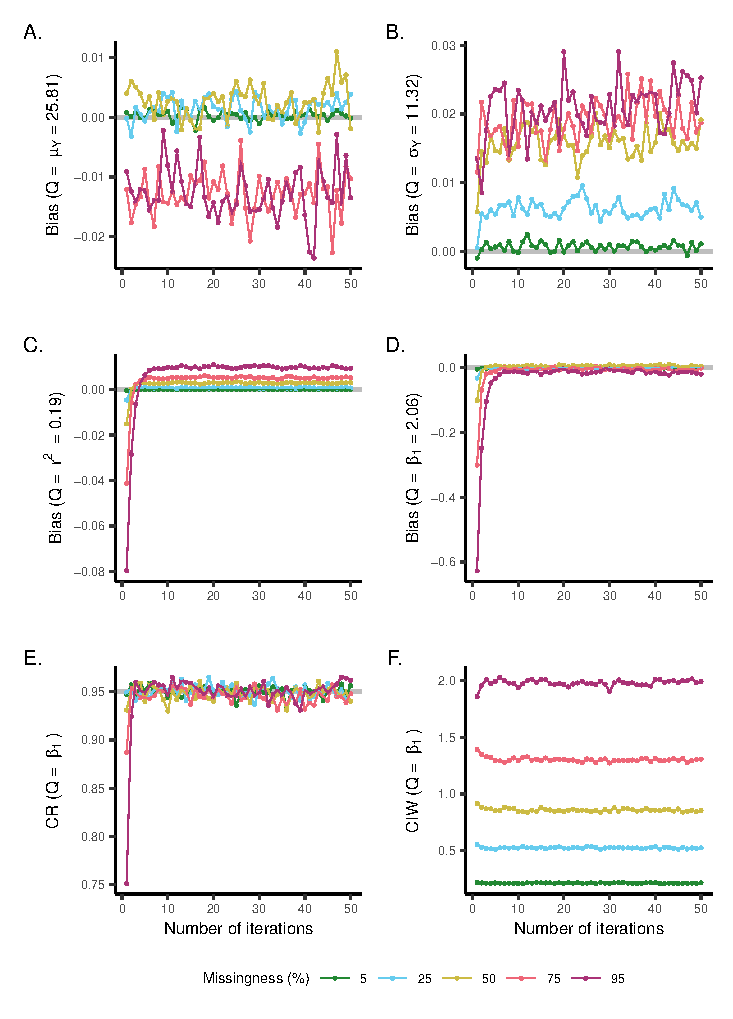
\includegraphics{2.Manuscript_files/figure-latex/Qs-1} 

}

\caption{Impact of non-convergence on statistical inferences.}\label{fig:Qs}
\end{figure}

Figure \ref{fig:Qs} displays the influence of inducing non-convergence on the estimated quantities of scientific interest, \(Q\)s. \textbf{{[}Add panel labels, describe panels{]}} As expected, conditions with a higher proportion of missingness and/or a lower number of iterations are impacted more severely by non-convergence. I.e., on average these conditions portray more extreme bias in the estimated \(Q\)s, and non-nominal coverages. Roughly speaking, this means that the algorithm is indeed not converged at \(t=1\), and converges gradually as \(t\) increases to \(T\). The point at which an additional iteration does not lead to an improvement in the estimates depends on quantity of scientific interest \(Q\) and the missingness proportion \(p_{mis}\). The highest number of iterations that is necessary to reach this point across all simulation conditions is \(T=7\). This implies that, under the current specifications, no more than seven iterations are necessary to obtain \emph{sufficient} performance in terms of bias and confidence validity.

\hypertarget{qmu.}{%
\subsubsection{\texorpdfstring{\(Q=\mu\).}{Q=\textbackslash mu.}}\label{qmu.}}

The estimated univariate means seem unaffected by the number of iterations in the algorithm. The magnitude of the bias in \(\bar{Q}\) depends exclusively on the missingness proportion \(p_{mis}\), with higher missingness proportions causing more extreme bias. Note however, that the simulation condition with the largest overall bias resulted in a \(\bar{Q}\) under-estimated the true value of \(Q\) by only 0.02 units (where \(Q=\mu_Y=25.81; \sigma_Y = 11.32\)). We conclude that---conditional on the missingness proportion---all simulation conditions (\(T \geq 1\)) have equal performance. According to this scientific estimand \(Q\), non-convergence does not impact the validity of the inferences. \textbf{{[}Add: up-to 50\% missingness everything is relatively unbiased, while 75\% and 95\% missingness show very different results. Why is that? Add sd of Y in the figure to show that the bias is relative: a bias of 0.02 for a variable with a mean of 25.81, and sd of 11.32 is nothing.{]}}

\hypertarget{qsigma.}{%
\subsubsection{\texorpdfstring{\(Q=\sigma\).}{Q=\textbackslash sigma.}}\label{qsigma.}}

The estimated standard deviations show impact of non-convergence similar to the means. The magnitude of the bias \(\bar{Q}\) follows the incremental order of the missingness proportions. The number of iterations in the algorithm has little effect on the bias. Only the estimates in simulation conditions with just one iteration (\(T=1\)) differ from other conditions that have the same missingness proportion but a higher number of iterations. Interestingly, the bias in conditions where \(T=1\) is \emph{less} severe than after continued iteration. For the least possible bias, we may use any number of iterations \(T\geq1\), but only \(p_{mis} = 0.05\) results in completely unbiased \(\bar{Q}\)s.

\hypertarget{qbeta.}{%
\subsubsection{\texorpdfstring{\(Q=\beta\).}{Q=\textbackslash beta.}}\label{qbeta.}}

For the estimated regression coefficients, we consider bias, confidence interval width (CIW), and coverage rate (CR) as performance measures. The magnitude of the bias, again, depends on the missingness proportion. But for this \(Q\) we also observe a clear effect of the number of iterations. Conditions with a lower number of iterations yield more bias in \(\bar{Q}\). This is especially pronounced in conditions with high missingness proportions: with 95\% missingness we need at least seven iterations before an additional iteration does not lead to improved estimates. Conditions with a lower missingness proportion (e.g., \(p_{mis} = {0.5}\)), produce \emph{optimal} estimates with as many as two iterations. Approximately unbiased estimates are obtained for all conditions where \(p_{mis}\leq0.75\) and \(T\leq6\). \textbf{{[}Add CIW and CR{]}}

\hypertarget{qr2.}{%
\subsubsection{\texorpdfstring{\(Q=r^2\).}{Q=r\^{}2.}}\label{qr2.}}

The bias in the estimated explained variance perfectly follows both sets of simulation conditions: The worst performance is observed for the highest missingness proportion and the lowest number of iterations, while the best performance occurs with less missingness and more iterations. Only conditions with the lowest missingness proportion (\(p_{mis}=0.05\)) results in unbiased estimates for every number of iterations. In other conditions there is at least some bias irrespective of \(T\). The inferences do not improve in any condition where \(T \geq 6\). This suggests that the algorithm is as converged as necessary to obtain valid inferences.

\hypertarget{non-convergence-diagnostics}{%
\subsection{Non-convergence diagnostics}\label{non-convergence-diagnostics}}

In Figure \ref{fig:rhats-acs} we see the results of the non-convergence diagnostics \(\widehat{R}\) and \(AC\). \textbf{{[}Add panel labels and explain how to read the plots{]}} As expected, the diagnostics identify more signs of non-convergence in simulation conditions with a lower number of iterations. The missingness proportions, however, only seem to impact multivariate convergence. When \(\widehat{R}\) and \(AC\) are applied to univariate \(\theta\)s, they identify the same amount of non-convergence, irrespective of the missingness proportion. When the diagnostics are applied to multivariate \(\theta\)s, they generally identify more signs of non-convergence for higher missingness proportions.

None of the simulation conditions that we consider resulted in complete convergence of the algorithm (defined as \(\widehat{R}=1\) and \(AC=0\)). The thresholds for diagnosing non-convergence that are used in practice seem too conservative compared to the performance measures: \(\widehat{R}\) and \(AC\) identify signs of non-convergence in conditions where the \(\bar{Q}\)s are unbiased and confidence valid estimates of the \(Q\)s. The most recent recommended threshold for diagnosing non-convergence with \(\widehat{R}\) is never overcome in this study (all \(\widehat{R}\)\textgreater1.01). Apparently, this threshold is too stringent for iterative imputation algorithms, and will not be discussed further.

\begin{figure}

{\centering 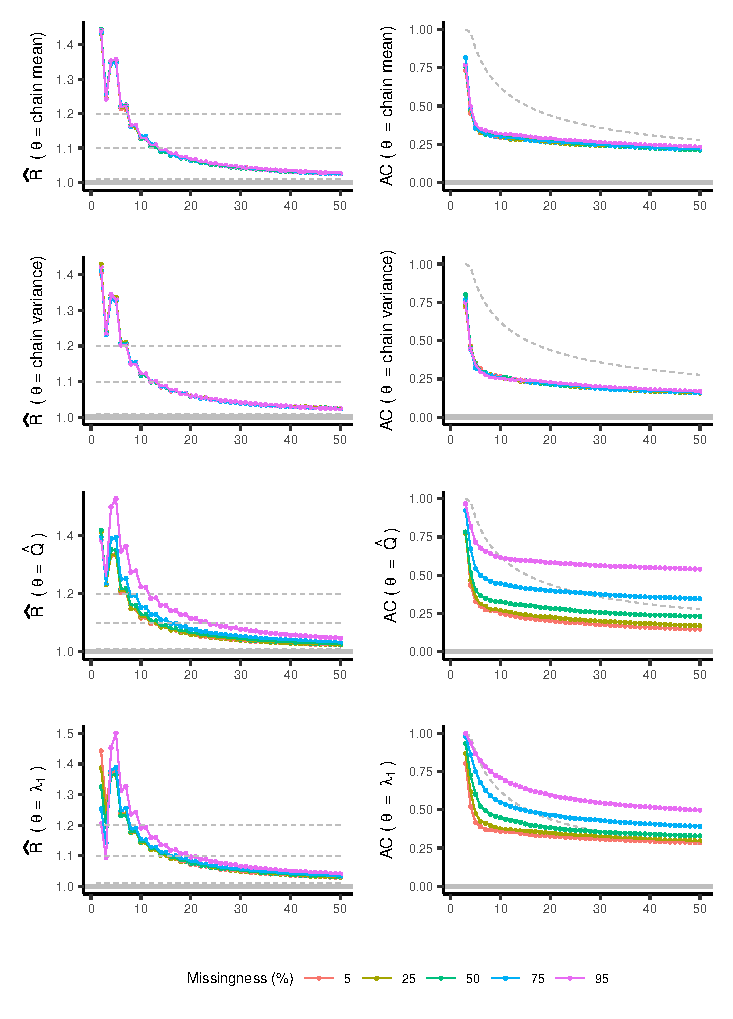
\includegraphics{2.Manuscript_files/figure-latex/rhats-acs-1} 

}

\caption{Non-convergence diagnostics. [Split up into 2 or 4 figures??]}\label{fig:rhats-acs}
\end{figure}

\hypertarget{theta-chain-mean.}{%
\subsubsection{\texorpdfstring{\(\theta=\) chain mean.}{\textbackslash theta= chain mean.}}\label{theta-chain-mean.}}

When \(\widehat{R}\) and \(AC\) are applied to the chain means, we notice no impact of the missingness proportions. The results only depend on the number of iterations per simulation condition.

\textbf{{[}MAYBE remove all this because it has no relation to the bias in Q{]} The highest \(\widehat{R}\)-values are obtained for the condition \(T=2\). We observe the same `dip' in \(\widehat{R}\) as we did in Figure \ref{fig:diagnostics} for conditions with three iterations. \(\widehat{R}\) gradually decreases as the number of iterations increases across conditions. By the traditional threshold \(\widehat{R}>1.2\) we should conclude that there is non-convergence in conditions where \(T<8\). The common threshold \(\widehat{R}>1.1\) is overcome in conditions where \(T>14\). }

\textbf{Autocorrelations indicate some signs of non-stationarity in all simulation conditions, but primarily in conditions where \(T<6\). The threshold for diagnosing non-convergence is not reached in any condition. We would thus conclude that the algorithm is sufficiently converged regardless of the number of iterations or missingness proportion. }

We evaluate the diagnostics with chain means as \(\theta\) against the bias in \(Q=\mu\). According to the bias in the univariate means, we should conclude that two iterations is sufficient, and we should see that \(p_{mis}=0.75\) and \(p_{mis}=0.95\) have worse convergence than the other missingness proportions. This is not the case.

\hypertarget{theta-chain-variance.}{%
\subsubsection{\texorpdfstring{\(\theta=\) chain variance.}{\textbackslash theta= chain variance.}}\label{theta-chain-variance.}}

The non-convergence diagnostics applied to the chain variances as \(\theta\) yield highly similar results to the chain means. We therefore evaluate these results immediately against the corresponding \(Q\), without describing the \(\widehat{R}\) and \(AC\) values. While the bias in the estimated standard deviations mainly depends on the missingness proportion of each condition, \(\widehat{R}\) and \(AC\) are influenced mostly by the number of iterations. We thus conclude that there is no added value of evaluating non-convergence with chain variances as \(\theta\) in the diagnostics.

\hypertarget{thetahatq.}{%
\subsubsection{\texorpdfstring{\(\theta=\hat{Q}\).}{\textbackslash theta=\textbackslash hat\{Q\}.}}\label{thetahatq.}}

The non-convergence diagnostics are applied to the estimated regression coefficients in each imputation, and evaluated against the bias in the corresponding pooled estimate.

\(\widehat{R}\) indicates signs of non-convergence across all missingness proportions and each number of iterations, in the expected order: simulation conditions with higher missingness proportions and less iterations are identified as the worst converged. The thresholds to diagnose non-convergence are overcome in different conditions, depending on the number of iterations and the missingness proportion. The most lenient threshold (\(\widehat{R}>1.2\)) is overcome at \(T\geq9\) for \(p_{mis} = 0.05\), and \(T\geq12\) for \(p_{mis} = 0.95\). The conventional \(\widehat{R}>1.1\) is surpassed at \(T\geq12\) and \(T\geq24\), respectively.

For the autocorrelations applied to the \(\hat{Q}\)s, we see an even stronger effect of the missingness proportions. Especially the conditions where \(p_{mis} = 0.75\) and \(p_{mis} = 0.95\) are identified as non-stationary. The threshold used to evaluate whether \(AC=0\), however, is only reached in conditions with at least ten iterations. This suggests that the default number of iterations may be too low to detect non-stationarity with \(AC\). However, the critical value for diagnosing non-convergence with \(AC\) decreases as a function of the number of iterations. The conclusion to identify non-stationarity in conditions where \(T\geq10\) and \(p_{mis} = 0.95\) might therefore be spurious. \textbf{{[}Also, the \(AC\) across missingness proportions shows the opposite of what you would expect: shouldn't there be higher autocorrelations in conditions with comparatively more observed data in the completed datasets? I don't understand this.{]}}

Compared to the bias in \(\bar{Q}\), the diagnostics applied to the \(\hat{Q}\)s over-estimate the severity of the non-convergence. This is odd, since the \(\theta\) and \(Q\) are directly related.

\hypertarget{thetalambda_1.}{%
\subsubsection{\texorpdfstring{\(\theta=\lambda_1\).}{\textbackslash theta=\textbackslash lambda\_1.}}\label{thetalambda_1.}}

Finally, we evaluate the non-convergence diagnostics applied to the first eigenvalue of the variance-covariance matrices of the completed data. Similar to the results the the regression coefficients as \(\theta\)s, we see effects of both the missingness proportion and number of iterations in each simulation condition. The most signs of non-convergence are identified in conditions where \(p_{mis}\) is large and \(T\) is small.

Notwithstanding the similarities with \(\theta=\hat{Q}\), there is a big difference in \(\widehat{R}\)-values for conditions where \(T<4\). In these conditions, \(\widehat{R}\) behaves oppositely of our expectation: conditions with the lowest missingness proportions yield the highest \(\widehat{R}\)-values. In conditions with a higher number of iterations, this artifact disappears. This suggests that the combination of \(\widehat{R}\) and \(\lambda_1\) is only appropriate for imputation algorithms where the number of iterations at least four. Interpreting the \(\widehat{R}\) values of conditions where \(T<3\) may lead to the incorrect conclusion that only conditions with \emph{low} missingness proportions show signs of non-convergence. For applications as a model-independent multivariate \(\theta\), we should therefore only interpret the \(\widehat{R}\)-values when \(T\geq4\). Using this cut-off we conveniently ignore the initial `dip' at \(T=3\) as well. The traditional threshold \(\widehat{R} > 1.2\) is overcome in conditions where \(p_{mis} = .95\) and \(T\geq10\), and for all other missingness proportions in conditions where \(T\geq8\). With the \(\widehat{R} > 1.1\) threshold, the number of iterations are \(T\geq20\) and \(T\geq16\), respectively.

The \(AC\)-values largely depend on the missingness proportion in each condition. Conditions where \(p_{mis}=.95\) show statistically significant autocorrelations for any number of iterations. The other extreme, conditions where \(p_{mis}=.05\), does not yield \(AC\) values above the threshold. The \(AC\) values with this missingness proportion are equivalent for all conditions where \(T\geq6\), which suggests that the algorithm is as stationary as it can be. A similar point is only observed after twenty iterations in conditions with higher missingness proportions.

In comparison to the \(Q\)s, the diagnostics again over-estimate the signs of non-convergence. Conditions with low missingness proportions (e.g., 5\% or 25\% of the complete data) yield unbiased, confidence valid estimates with as little as two iterations. The convergence diagnostics, however, indicate improved convergence up-to eight iterations according to \(AC\) and thirty to forty iterations according to \(\widehat{R}\). The model-independent \(\theta\) \(\lambda_1\) seems as well-equipped to diagnose signs of non-convergence as \(\theta=\hat{Q}\). The univariate \(\theta\)s do not differentiate between bias induced by the missingness proportions.

\hypertarget{in-short-remove-later}{%
\subsection{In short {[}remove later!{]}}\label{in-short-remove-later}}

\begin{itemize}
\item
  Is there more bias in conditions where non-convergence was induced? (NOPE for univariates, YES for multivar.).
\item
  Is the point of \emph{sufficient} convergence (at which the \(\bar{Q}\)s are unbiased and confidence valid estimates of the \(Q\)s) the same point as identified by the non-convergence diagnostics? (NOPE, they are too conservative).
\item
  Is one of the thetas better? (YES, while it doesn't really matter as long as it's multivariate, \(\lambda_1\) is model-independent and therefore preferred).
\item
  What should the thresholds be? (much HIGHER than recommended for \(\widehat{R}\), difficult to say for \(AC\)).
\item
  And the default nr of iterations? (MAYBE increase to 10 to detect significant \(AC\) and be sure not to miss the dip in \(\widehat{R}\)?).
\end{itemize}

\hypertarget{discussion}{%
\section{Discussion}\label{discussion}}

In short, iterative imputation algorithms may yield approximately unbiased, confidence valid estimates under different levels of induced non-convergence. Univariate estimates seem robust against terminating the algorithm early: There is no clear effect of the number of iterations on the bias in estimated means and standard deviations. The bias in these \(Q\)s was only impacted by the missingness proporion \(p_{mis}\), with higher \(p_{mis}\) resulting in more bias. Bias in multivariate estimates depended on both \(p_{mis}\) and the number of iterations. However, the only effect of the number of iterations was observed when the algorithm was terminated at seven iterations or earlier. This suggests that continued iteration beyond seven iterations does not yield better estimates. Yet, the non-convergence diagnostics \(\widehat{R}\) and \(AC\) indicated that the iterative imputation algorithm did not reach a stable state before twenty to thirty iterations. \textbf{{[}MERGE or remove{]} \(\widehat{R}\) and autocorrelation indicate that there are signs of non-convergence in the algorithm up-to at least twenty iterations, while unbiased, confidence valid estimates may be obtained with as little as one iteration. This observation is in agreement with }one of {[}still add the others!{]}** the simulation hypotheses: \(\widehat{R}\) over-estimates the severity of non-convergence when applied to MI procedures.**

Over-estimation of the signs of non-convergence may be due to the methods (and their thresholds) or due to the \(Q\)s (descriptive and multivariate linear regression, not higher dimensional/more complex \(Q\)s). More complicated \(Q\)s (e.g., higher-order effects or variance components) might show bias, under- or over-coverage at higher \(T\). Which might be why \(\widehat{R}\) and \(AC\) identify non-convergence.

\hypertarget{recommendations-for-empirical-researchers}{%
\subsection{Recommendations for empirical researchers}\label{recommendations-for-empirical-researchers}}

For empirical researchers:

\begin{enumerate}
\def\labelenumi{\arabic{enumi}.}
\item
  Check traceplots for signs of pathological non-convergence. Adjust imputation model if necessary.
\item
  Monitor non-convergence diagnostics \(\widehat{R}\) and \(AC\). Use the thresholds for \(\widehat{R}>1.2\) and autocorrelation \textbf{???}. Keep iterating until these thresholds are reached.
\item
  Do not use the traditional calculation for \(\widehat{R}\), or the \texttt{R} function \texttt{stats::acf()} to compute \(AC\). Instead, calculate \(\widehat{R}\) conform \citet{veht19} and compute autocorrelations manually (see e.g., \href{https://github.com/gerkovink/shinyMice/tree/master/3.Thesis/1.SimulationStudy}{github.com/gerkovink/shinyMice}).
\item
  Track your own scalar summary of interest (see e.g., \citet{buur18}). Compute \(\widehat{R}\) and autocorrelation values for this scalar summary.
\item
  \textbf{Something} about the novel \(\theta\) that is `substantive model-independent'.
\end{enumerate}

\hypertarget{recommendations-for-future-research}{%
\subsection{Recommendations for future research}\label{recommendations-for-future-research}}

Further research is needed to investigate the performance of iterative imputation algorithms under clear violation of convergence, e.g.~dependency between predictors (predictors with very high correlations). For example:

\begin{itemize}
\item
  Induce non-convergence with mis-specified imputation model.
\item
  Introduce more difficult missingness problems, i.e., M(N)AR instead of MCAR. That is, proper performance under a `missing completely at random' missingness mechanism is necessary to demonstrate the appropriateness of \(\widehat{R}\) and \(AC\) as non-convergence diagnostics. However, results may not be extrapolated to other missingness mechanisms.
\item
  Imputation technique with questionable convergence properties, e.g., PMM.
\item
  Apply recommendations to empirical data and write a vignette for applied researchers.
\item
  Implement recommendations in ShinyMICE.
\item
  Develop an additional convergence diagnostic unique for iterative imputation: \(AC\) across imputations, instead of iterations.
\end{itemize}

In short, we have shown that an iterative imputation algorithm can yield correct outcomes, even when a converged state is not reached according to two common non-convergence diagnostics. Continued iteration just burns a lot of computing time, without improving the statistical inferences. To conclude, in the case of drawing inference from incomplete data, convergence of the iterative imputation algorithm is often a convenience but not a necessity.

\bibliographystyle{sageh}
\bibliography{thesis.bib}


\end{document}
